\section{Технологический раздел}
%В этом разделе рассматривается выбор средств реализации, описывается структура классов программы и описывается интерфейс программного обеспечения.

\subsection{Средства реализации}
\subsubsection{Выбор языка программирования}
Для написания данной курсовой работы был выбран язык C\#~\cite{cpp-lang}.
Этот выбор обусловлен следующими причинами:
\begin{itemize}
	\item C\# --- объектно-ориентированный язык, что соответствует методологии, выбранной для разработки программы;
	\item C\# предоставляется обширный набор библиотек и шаблонов, что позволяет использовать готовые конструкции и значительно экономит время разработки.
\end{itemize}

В качестве среды разработки был использован Visual Studio 2022~\cite{qt-creator}.
Данный выбор обусловлен следующими факторами:
\begin{itemize}
	\item в Visual Studio есть возможность быстрого создания интерфейса с помощью WinForms;
	\item Visual Studio предоставляет шаблоны, которые облегчают процесс написания и отладки проекта.
\end{itemize}

\subsubsection{Выбор СУБД}
Рассматриваются некоторые полулярные реляционные СУБД \cite{dbms}:
\begin{itemize}
	\item Oracle;
	\item My SQL;
	\item Microsoft SQL Sever;
	\item PostgreSQL.
\end{itemize}
Выделяются следующие критерии для сравнения перечисленных СУБД:
\begin{itemize}
	\item Лицензия;
	\item Возможность создания роли, выдачи права на уровне БД;
	\item Масштабируемость;
	\item Сообщество и подержка;
\end{itemize}

\begin{table}[h!]
	\begin{center}
		\caption{Сравнение реляционных СУБД \cite{dbms}}
		\label{tab:comparison}
		\begin{tabular}{|l|c|c|c|c|}
			\hline
			& Oracle & MySQL & MSQL Server & PostgreSQL \\
			\hline
			Лицензия & Коммер. & Двойная & Коммер. & Открытая \\
			Создания ролей & Да & Да & Да & Да \\
			Масштабируемость & Высокая & Хорошая & Хорошая & Высокая \\
			Сообщ. и поддержка & Крупное & Активное & Обширное & Крупное \\
			\hline
		\end{tabular}
	\end{center}
\end{table}

Исходя из сравнения по этим критериям, PostgreSQL представляется привлекательным выбором ввиду своей открытой лицензии, богатых возможностей управления ролями и правами доступа, высокой масштабируемости и активного сообщества с открытым исходным кодом, что делает его привлекательным для разнообразных проектов и бизнесов.

\subsection{Создание базы данных}
На основе ER-диагрммы базы данных, представленной на рисунке \ref{img:ERD} были созданы все сущности. Программный код приведен в листинге \ref{lst:createtable} в приложении A.

Была создана ролевая модель на листингах \ref{lst:role1}--\ref{lst:role5} в приложении A.

Реализация функций на листинге \ref{lst:f1} в приложении A.
Реализация триггера на листинге \ref{lst:trigger} в приложении A.

\subsection{Описание интерфейсов}
Проект ориентирован на создание удобного и интуитивно понятного пользовательского интерфейса для работы с базой данных через Desktop-приложение.
Он предоставляет пользователям простой и интуитивно понятный способ нахождения необходимой информации и выполнения требуемых операций.
На рисунках \ref{img:ex1}--\ref{img:ex6} в приложении A, отображают интерфейсы, которые были спроектированы для обеспечения этой цели.
В этих изображениях могут быть показаны компоненты, предоставляющие пользователям возможность взаимодействия с данными из базы данных.

\subsection{Тестирование}
\subsubsection{Функция}
Проводится тестирования функции, которая составляет турнирную таблицу на следующих случаях:
\begin{enumerate}
	\item Турнир состоит из 6 команд, все матчи сыграны.
	\item Турнир состоит из 4 команды, часть матчей сыграна.
	\item Турнир состоит из 4 команды, матчи не были сыграны.
\end{enumerate}

Реализация тестирования приведена в листинге \ref{lst:test1} в приложении A.

На рисунке \ref{img:testfunction} приведены результаты тестирования.
\begin{figure}[h]
	\centering
	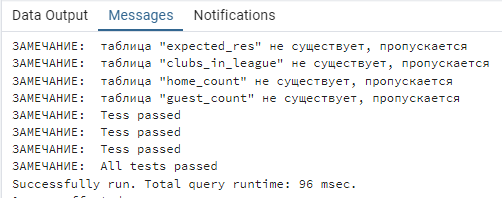
\includegraphics[height=0.2\textheight]{img/testfunction.png}
	\caption{Результаты тестов для функции get\_table()}
	\label{img:testfunction}
\end{figure}

\subsubsection{Триггер}
Проводится тестирования триггер, который автоматически обновляет значение поля <<rating>> в таблице leagues при добавлении новых оценок на следующих случаях:
\begin{enumerate}
	\item Добавление средней оценки.
	\item Добавление нижней граничной оценки.
	\item Добавление верхней граничной оценки.
\end{enumerate}

Реализация тестирования приведена в листинге \ref{lst:test2} в приложении A.

На рисунке \ref{img:testtrigger} приведены результаты тестирования.
\begin{figure}[h]
	\centering
	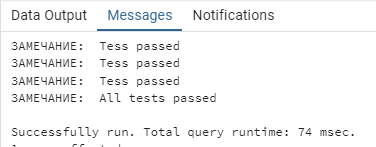
\includegraphics[height=0.2\textheight]{img/testtrigger.png}
	\caption{Результаты тестов для триггера auto\_cal\_rating}
	\label{img:testtrigger}
\end{figure}
\subsection*{Вывод}
Был рассмотрен выбор средств реализации, описан интерфейс программного обеспечения и проведено тестирование функции на строне базы данных.
